%% UniAgent (ICCCM 2026) -- built on the ACM "acmart" sigconf template.
%% For double-anonymous review, change the documentclass line to
%% \documentclass[sigconf, anonymous, review]{acmart}.
%TC:macro \cite [option:text,text]
%TC:macro \citep [option:text,text]
%TC:macro \citet [option:text,text]
%TC:envir table 0 1
%TC:envir table* 0 1
%TC:envir tabular [ignore] word
%TC:envir displaymath 0 word
%TC:envir math 0 word
%TC:envir comment 0 0
% !TeX root = sample-sigconf.tex
\documentclass[sigconf]{acmart}

\AtBeginDocument{%
  \providecommand\BibTeX{{%
    Bib\TeX}}}

%% Figure assets live in paper/images/
\graphicspath{{images/}}
\usepackage{subcaption}
\usepackage{cuted}

%% Give LaTeX more freedom when placing floats so that figures and tables
%% stay on (or nearer) the page that references them instead of drifting.
\setcounter{topnumber}{3}
\setcounter{bottomnumber}{2}
\setcounter{totalnumber}{4}
\setcounter{dbltopnumber}{3}
\renewcommand{\topfraction}{0.92}
\renewcommand{\bottomfraction}{0.5}
\renewcommand{\dbltopfraction}{0.92}
\renewcommand{\textfraction}{0.07}
\renewcommand{\floatpagefraction}{0.72}
\renewcommand{\dblfloatpagefraction}{0.72}

%% dblfloatfix corrects the placement order of deferred double-column
%% (table*/figure*) floats and enables bottom [b] placement, so a wide
%% table is not stranded on the last page above the references.
\usepackage{dblfloatfix}

%% placeins/\FloatBarrier lets us keep a float inside the section that
%% references it (used to pin the comparison table to the Evaluation
%% section instead of letting it drift past the references).
\usepackage{placeins}

%% Rights management information. Replace the SAMPLE values below with
%% the commands provided when the rights form is completed.
\setcopyright{acmlicensed}
\copyrightyear{2026}
\acmYear{2026}
\acmDOI{XXXXXXX.XXXXXXX}
%% ICCCM 2026 proceedings DOI is assigned by ACM after publication.
\acmConference[ICCCM '26]{The 14th International Conference on Computer and Communications Management (ICCCM 2026)}{July 24--26, 2026}{Tokyo, Japan}
\acmISBN{979-8-4007-2439-8}

\begin{document}

\title[UniAgent: End-to-End Decentralized Agent Framework]{UniAgent: An End-to-End Decentralized Framework for Autonomous Agent Discovery, Delegation, and Payment}

\author{Ryoto Taga}
\email{ryoto.taga12@gmail.com}
\affiliation{%
  \institution{Independent Researcher}
  \city{Tokyo}
  \country{Japan}
}
\author{M. Fahim Ferdous Khan}
\email{khan@iniad.org}
\affiliation{%
  \institution{Faculty of Information Networking for Innovation and Design (INIAD)}
  \institution{Toyo University}
  \city{Tokyo}
  \country{Japan}
}

\renewcommand{\shortauthors}{Taga and Khan}

\begin{abstract}
  Large language model (LLM) agents are increasingly able to act on
  behalf of users, but the infrastructure that lets them find, hire,
  and pay one another across organizational boundaries is still
  fragmented. Open protocols already exist for the individual pieces:
  the Agent2Agent (A2A) protocol standardizes agent-to-agent
  communication, x402 turns the HTTP~402 status code into a
  micropayment channel, and ERC-8004 records agent identity on chain.
  However, these protocols have so far been demonstrated only in
  isolation or as one-to-one proofs of concept, and no end-to-end
  service architecture ties them together so that a single
  natural-language request is autonomously decomposed into agent
  discovery, delegation, and payment. In this paper we present
  \emph{UniAgent}, a decentralized agent marketplace that integrates
  A2A, x402, and ERC-8004 under an LLM-based orchestration layer. A
  three-layer design separates a \emph{marketplace layer} (an on-chain
  ERC-8004 registry kept in sync with an off-chain cache through
  blockchain event webhooks), an \emph{orchestration layer} (a ReAct
  agent that discovers, inspects, and invokes external agents through
  three tools), and a \emph{payment layer} (x402 with delegated
  signing). We describe a working
  prototype deployed on the Base Sepolia testnet and report an
  end-to-end evaluation over 20 flight- and hotel-search tasks. UniAgent
  shows that open communication, on-chain identity, and
  protocol-native micropayments can be combined into a coherent,
  vendor-neutral marketplace in which user tasks are carried out
  across separately deployed A2A services.
\end{abstract}

\begin{CCSXML}
<ccs2012>
 <concept>
  <concept_id>10010147.10010178.10010179</concept_id>
  <concept_desc>Computing methodologies~Multi-agent systems</concept_desc>
  <concept_significance>500</concept_significance>
 </concept>
 <concept>
  <concept_id>10002951.10003260.10003282</concept_id>
  <concept_desc>Information systems~Web services</concept_desc>
  <concept_significance>300</concept_significance>
 </concept>
 <concept>
  <concept_id>10003752.10010124.10010131</concept_id>
  <concept_desc>Software and its engineering~Distributed systems organizing principles</concept_desc>
  <concept_significance>300</concept_significance>
 </concept>
</ccs2012>
\end{CCSXML}

\ccsdesc[500]{Computing methodologies~Multi-agent systems}
\ccsdesc[300]{Information systems~Web services}
\ccsdesc[300]{Software and its engineering~Distributed systems organizing principles}

\keywords{AI agents, agent marketplace, A2A protocol, x402, ERC-8004,
  micropayments, on-chain identity, LLM orchestration, ReAct}

\maketitle

\section{Introduction}
\label{sec:introduction}

Large language models (LLMs) have made it practical to build
autonomous agents that plan, call tools, and complete multi-step tasks
on behalf of a user. As these agents proliferate, a natural next step
is for one agent to delegate work to another: a travel assistant might
hire a specialized flight agent and a separate hotel agent, each
operated by a different organization. Realizing this vision requires
three capabilities that cut across trust boundaries: agents must be
able to \emph{communicate} with one another, to be \emph{discovered}
and \emph{identified}, and to \emph{pay} for services without a shared
account or a manual contract.

Open standards have recently emerged for each of these capabilities.
The Agent2Agent (A2A) protocol~\cite{a2a2025} defines how agents
describe themselves through an \emph{Agent Card} and exchange messages
over JSON-RPC. The x402 protocol~\cite{x402whitepaper} reuses the long-dormant
HTTP~402 ``Payment Required'' status code to attach stablecoin
micropayments to ordinary web requests. ERC-8004~\cite{erc8004}
provides an on-chain registry of agent identities, building on the
ERC-721 token standard so that any party can look up an
agent without trusting a central directory. Individually, these
protocols are compelling; together, they suggest a decentralized
alternative to the closed agent stores offered by today's platforms.

Despite this progress, three gaps remain. \textbf{First}, A2A
standardizes communication but explicitly leaves \emph{discovery}---how
a client finds an appropriate agent in the first place---outside its
scope. \textbf{Second}, recent work by Vaziry et
al.~\cite{vaziry2025} demonstrated the technical feasibility of
combining A2A, x402, and on-chain Agent Cards, but did so at the
protocol level, as one-to-one interactions between a fixed pair of
agents; it did not provide a service architecture that takes a
user's high-level task and autonomously drives discovery, delegation,
and payment to completion. \textbf{Third}, centralized platforms such
as the OpenAI GPT Store~\cite{gptstore} do offer end-to-end
experiences, but they confine the agent ecosystem to plug-ins inside a
single vendor's walled garden~\cite{frieden2016platforms}, with
platform-specific registration, discovery, and billing.

The result is a missing middle: the individual protocols exist, and
closed platforms show what a smooth user experience looks like, but no
\emph{open} architecture connects the protocols through an
orchestration layer that can turn a natural-language request into
cross-organizational agent transactions. This motivates our research
question:

\begin{quote}
\itshape How can open agent communication, on-chain identity, and
protocol-level micropayments be integrated into a cohesive marketplace
architecture with LLM-based orchestration, so that a user's high-level
task is autonomously decomposed into agent discovery, delegation, and
payment across organizational boundaries?
\end{quote}

We answer this question with \emph{UniAgent}, a decentralized agent
marketplace whose architecture is summarized in
Figure~\ref{fig:arch}. UniAgent takes the registration, discovery, and
payment functions that a centralized platform bundles together and
re-implements them on open protocols---A2A and x402---and a
standardized on-chain identity layer---ERC-8004. On top of these, an
LLM ReAct agent~\cite{yao2023react} acts as an orchestration layer that
analyzes the task, discovers candidate agents, inspects their
specifications, selects among them, and executes them with automatic
payment.

\paragraph{Contributions.} This paper makes three contributions:
\begin{enumerate}
  \item \textbf{An integrated marketplace architecture} that unifies
    A2A, x402, and ERC-8004 behind an orchestration layer, organized
    as three loosely coupled layers (marketplace, orchestration,
    payment).
  \item \textbf{An autonomous LLM pipeline} in which a ReAct agent
    drives task analysis, agent discovery, specification inspection,
    and paid execution through three tools (\texttt{discover\_agents},
    \texttt{fetch\_agent\_spec}, and
    \texttt{execute\_and\_evaluate\_agent}).
  \item \textbf{A working prototype and end-to-end
    demonstration}\footnote{Source code:
    \url{https://github.com/toryoto/UniAgent}; live demo:
    \url{https://uni-agent-web.vercel.app/}.} on
    the Base Sepolia testnet, exercising the full flow over external
    flight- and hotel-search services and reporting end-to-end success
    rate.
\end{enumerate}

The rest of the paper is organized as follows.
Section~\ref{sec:background} reviews the protocols UniAgent builds on.
Section~\ref{sec:related} positions our work against related research,
with particular attention to Vaziry et al.
Section~\ref{sec:architecture} presents the three-layer architecture,
the core of our contribution. Section~\ref{sec:implementation}
describes the prototype, and Section~\ref{sec:evaluation} evaluates it.
Section~\ref{sec:discussion} discusses limitations and future work, and
Section~\ref{sec:conclusion} concludes.

\section{Background}
\label{sec:background}

UniAgent builds on four open technologies.
The \emph{Agent2Agent (A2A)} protocol~\cite{a2a2025} standardizes
inter-agent communication: each agent publishes an Agent Card at a
well-known URL describing its capabilities and endpoint, and clients
exchange tasks over JSON-RPC. A2A deliberately leaves agent
\emph{discovery} outside its scope.
The \emph{x402} protocol~\cite{x402whitepaper} revives the HTTP~402
status code for micropayments: a server responds with payment
requirements, the client signs a stablecoin transfer, and a facilitator
settles the transaction on chain.
\emph{ERC-8004}~\cite{erc8004} provides an on-chain agent identity
registry built on ERC-721, assigning each agent a token whose metadata
is stored off chain; because the registry is a public contract, any
client can enumerate agents without trusting a central catalog.
Finally, the \emph{ReAct} pattern~\cite{yao2023react} interleaves LLM
reasoning and tool calling, which suits orchestration where the set of
agents and prices must be explored at run time.

\section{Related Work}
\label{sec:related}

\paragraph{Agent communication protocols.}
Several protocols now compete to standardize how agents interact.
Ehtesham et al.~\cite{ehtesham2025survey} survey this space and compare
the Model Context Protocol (MCP), which connects a single
agent to tools and data sources, with peer-to-peer protocols such as
A2A and the Agent Network Protocol (ANP). UniAgent adopts A2A for
inter-agent communication because it is designed for cross-organization
delegation, and uses an MCP-style tool interface only \emph{inside} the
orchestrator. None of these communication protocols specifies discovery
or payment, which is precisely what our marketplace layer adds.

\paragraph{Agent payment systems.}
x402~\cite{x402whitepaper} attaches stablecoin transfers to ordinary
HTTP requests and settles them on a smart-contract chain. We build on
x402 because it is open, HTTP-native, and requires no proprietary
intermediary, and we extend it with delegated signing through Privy
(Section~\ref{sec:payment-layer}).

\paragraph{Decentralized agent identity and closest prior work.}
Vaziry et al.~\cite{vaziry2025} represent each agent's card as an
individual smart contract and show that A2A, x402, and on-chain identity
can interoperate. UniAgent instead consolidates identities into a single
standardized ERC-8004 registry~\cite{erc8004} rather than per-agent
contracts, and---more importantly---builds a full marketplace and
orchestration layer on top, as detailed below.

\paragraph{Difference from Vaziry et al.}
Table~\ref{tab:vaziry} summarizes the contrast.

\begin{table}[H]
  \caption{UniAgent compared with Vaziry et al.~\cite{vaziry2025}.}
  \label{tab:vaziry}
  \small
  \begin{tabular}{@{}p{0.20\linewidth}p{0.33\linewidth}p{0.33\linewidth}@{}}
    \toprule
    Aspect & Vaziry et al. & UniAgent \\
    \midrule
    Positioning & Protocol-level feasibility study
      & Marketplace architecture integrating the protocols \\
    Identity & Per-agent smart contracts
      & Single ERC-8004 standard registry \\
    Discovery & Four methods proposed, not integrated
      & Registry plus webhook-synced cache \\
    Payment & x402 over A2A, demonstrated
      & x402 with delegated signing \\
    Orchestration & None (fixed agent A\,$\to$\,B)
      & LLM ReAct agent discovers, selects, executes \\
    User experience & Protocol-level proof of concept
      & Chat UI and SSE streaming \\
    \bottomrule
  \end{tabular}
\end{table}

Vaziry et al. establish the technical \emph{feasibility} of the
protocol combination through one-to-one agent interactions. UniAgent
treats those protocols as building blocks and contributes the missing
layer above them: an LLM orchestrator that, given a single user task,
autonomously discovers agents from a standardized registry, selects
among them, pays them over x402, and returns an integrated
result---together with the user-facing experience (chat and streaming)
that this requires.

\paragraph{LLM multi-agent orchestration.}
AutoGen~\cite{wu2023autogen} shows how multiple LLM-based agents can
coordinate through conversation, tool use, and optional human input
within an application. UniAgent addresses a different layer: it treats
the marketplace itself---open registration, cross-vendor discovery, and
protocol-native payment---as the object of orchestration.

\paragraph{Centralized marketplaces.}
Centralized agent stores such as the OpenAI GPT Store~\cite{gptstore}
offer registration, discovery, and billing as a smooth, integrated
experience, but only within one vendor's platform: agents are listed,
ranked, and charged according to platform-specific rules, and there is
no portability across providers. Enterprise vendors are moving in the
same direction: Oracle AI Agent Marketplace embeds validated,
partner-built agent templates directly inside Oracle Fusion
Applications and adopts A2A for agent interoperability within that
environment~\cite{oracleAgentMarketplace2025}. Such systems reinforce
the demand for agent marketplaces, but they also show why A2A alone is
insufficient: communication may be standardized while registration,
discovery, deployment, and billing remain confined to a single vendor's
application layer. They also rely on platform-managed billing rather
than protocol-native micropayments. This resembles the broader platform
pattern of walled gardens, where openness and neutrality are limited by
the platform
operator~\cite{frieden2016platforms}. UniAgent aims to reproduce the
convenience of such platforms while keeping each function open and
vendor-neutral.

\section{System Architecture}
\label{sec:architecture}

UniAgent is organized into three layers, shown together in
Figure~\ref{fig:arch}: a \emph{marketplace layer} that maintains the
catalog of available agents, an \emph{orchestration layer} that turns a
user task into a sequence of agent invocations, and a \emph{payment
layer} that settles each invocation. The layers are deliberately
decoupled---the orchestrator does not need to know how identity is
stored, and the payment layer does not need to know why an agent was
selected---so that each can evolve independently. We describe each layer
in turn and then explain how they combine into an end-to-end flow.

\begin{figure*}[t]
  \centering
  
\includegraphics[width=\textwidth]{uniagent-system-arch}
  \caption{Overview of the UniAgent architecture. A user issues a
    natural-language task through the web application; an LLM-based
    agent service discovers candidate agents from an ERC-8004 registry
    (cached in PostgreSQL via Alchemy webhooks), invokes the selected
    external A2A agents, and settles payment over x402 using USDC on
    Base Sepolia.}
  \Description{A block diagram with three groups. On the left, a user
    in a browser connects through Privy to the UniAgent application,
    which contains a web app, an agent service, and a PostgreSQL cache.
    The agent service calls the Anthropic Claude API for reasoning and
    communicates with an external A2A agent. On the right, a Base
    Sepolia group contains the EAS, USDC, AgentStaking, and the
    ERC-8004 AgentIdentityRegistry contracts. Arrows show a chat
    execution flow and a marketplace synchronization flow driven by
    Alchemy webhooks and agent-developer registration.}
  \label{fig:arch}
\end{figure*}

\subsection{Marketplace Layer}
\label{sec:marketplace-layer}

The marketplace layer answers a single question: which agents exist and
what can they do? Its authoritative source is the on-chain ERC-8004
\texttt{AgentIdentityRegistry}. An agent developer deploys an A2A
agent, uploads its Agent Card to IPFS, and registers it in the registry
with the IPFS content identifier as the token's metadata URI, optionally
staking a deposit. Reading the chain on every request would be slow and
costly, so UniAgent maintains an off-chain PostgreSQL cache synchronized
through blockchain event webhooks: registration and staking events
trigger a webhook that fetches the metadata from IPFS and updates the
cache. The marketplace UI reads from this cache, while the chain remains
the single source of truth.

\subsection{Orchestration Layer}
\label{sec:orchestration-layer}

The orchestration layer is a ReAct agent~\cite{yao2023react} built with
LangChain and driven by a commercial LLM. It receives the user's
natural-language task and operates the marketplace through three tools:

\begin{sloppypar}
\begin{itemize}
  \item \texttt{discover\_agents(category, query)} returns a short list
    of candidate agents for a given need, drawn from the marketplace
    cache (Section~\ref{sec:marketplace-layer}).
  \item \texttt{fetch\_agent\_spec(agentId)} retrieves the candidate's
    Agent Card from its well-known URL and, when available, its OpenAPI
    specification. This lookup is free of charge and lets the LLM
    inspect skills, input modes, endpoint details, and x402 pricing
    before committing to a paid call.
  \item \texttt{execute\_and\_evaluate\_agent(agentId, category,
    input)} invokes the chosen agent over A2A, settles payment over
    x402 (Section~\ref{sec:payment-layer}), verifies the resulting
    on-chain transaction, and records a quality attestation through EAS.
\end{itemize}
\end{sloppypar}

\paragraph{Orchestration loop.}
Given a task such as planning a trip, the ReAct agent first decomposes
it into sub-tasks (e.g., a flight search and a hotel search). For each
sub-task it calls \texttt{discover\_agents} to obtain up to three ranked
candidates, then typically calls \texttt{fetch\_agent\_spec} on the most
promising ones to compare capabilities and prices. After selecting an
agent, it calls \texttt{execute\_and\_evaluate\_agent}, observes the
result, and repeats the loop until the overall task is complete, at which
point it composes a final answer. Crucially, the model is never given a fixed
plan or a hard-coded list of agents---both the decomposition and the
choice of providers emerge from the ReAct loop at run time.

\paragraph{Discovery ranking.}
To keep the candidate list short and useful, \texttt{discover\_agents}
does not return every matching agent. Instead, the marketplace ranks
candidates from the cache using a composite score that combines an
agent's reliability and quality (estimated from past attestations), the
size of its on-chain deposit, and a small bonus for newly registered
agents, and returns the top three. The reliability and quality
estimates are smoothed toward a global average so that agents with few
reviews are neither unfairly promoted nor permanently excluded
(mitigating the cold-start problem), and a small exploration term
occasionally surfaces a new agent so that it can accumulate a track
record. We describe the ranking qualitatively here, as a way to give the
LLM a manageable and balanced set of options; its exact form is an
engineering parameter rather than a contribution of this paper.

\subsection{Payment Layer}
\label{sec:payment-layer}

The payment layer settles each paid invocation using the x402
verify-and-settle pattern~\cite{x402whitepaper}. When the orchestrator
calls an external A2A agent, the agent responds with HTTP~402 and a
\texttt{PAYMENT-REQUIRED} header specifying the price and recipient. The
agent service obtains a delegated payment signature from a Privy wallet
without exposing the user's private key, and retries the request with
the signed payload. The external agent verifies and settles the payment
through an x402 facilitator, which submits the USDC transfer on chain.
The main UniAgent extension to the standard x402 pattern is
\emph{delegated signing} through Privy, which makes payments gasless and
non-custodial. After a successful execution, the system records an
off-chain quality and reliability attestation using the Ethereum
Attestation Service (EAS)~\cite{eas}; these attestations feed back into
the discovery ranking, closing the loop between payment and reputation.

\subsection{Integration Design}
\label{sec:integration-design}

After the user authenticates with Privy and submits a task, the web
application opens a server-sent events (SSE) stream and forwards the
task to the orchestrator. The orchestrator runs the ReAct
loop---discovering agents (marketplace layer), inspecting their Agent
Cards, and executing the chosen agent with x402 payment (payment
layer). Intermediate events---reasoning steps, tool calls, payments,
and partial results---are streamed back to the UI over SSE.

The value of the design comes from the combination rather than any
single protocol. A2A makes agents callable across organizations;
ERC-8004 makes them discoverable without a central directory; x402
makes them payable with a single signed request; and the orchestration
layer ties these together so that a user expresses a goal in natural
language and the system carries out discovery, delegation, and payment
automatically.

\section{Implementation}
\label{sec:implementation}

We implemented UniAgent as a TypeScript monorepo; the source code is
available at \url{https://github.com/toryoto/UniAgent} and the live
deployment at \url{https://uni-agent-web.vercel.app/}. The web application
uses Next.js and React, with Privy for social login and delegated wallets.
The orchestration service runs separately on LangChain with a commercial
LLM, exposing the three tools described in
Section~\ref{sec:orchestration-layer} and streaming results over SSE.
The marketplace cache is stored in PostgreSQL and accessed through an
ORM, with all database access confined to a dedicated data-access layer.
Smart contracts are written in Solidity and developed with Hardhat.
Payments use the x402 protocol with USDC on the Base Sepolia testnet.

\paragraph{Deployment.}
The prototype runs on the Base Sepolia testnet (chain ID~84532).
Table~\ref{tab:deployment} lists the main on-chain components: the
ERC-8004 \texttt{AgentIdentityRegistry} that anchors agent identity, the
\texttt{AgentStaking} contract that holds agent deposits, and the EAS
schema used to record per-interaction quality
and reliability attestations.

\begin{table}[H]
  \caption{Primary on-chain deployments (Base Sepolia, chain ID~84532).}
  \label{tab:deployment}
  \small
  \setlength{\tabcolsep}{4pt}
  \begin{tabular}{@{}lp{0.52\linewidth}@{}}
    \toprule
    Contract & Address \\
    \midrule
    AgentIdentityRegistry
      & \texttt{0x864A0C05\allowbreak 4AA6E9DBcC\allowbreak DB36a44a14\allowbreak A5A7bc81EB\allowbreak 92} \\
    AgentStaking
      & \texttt{0xC034e56E\allowbreak De7FC31579\allowbreak E41095A4e9\allowbreak 63D499e85d\allowbreak 39} \\
    \bottomrule
  \end{tabular}
\end{table}

\paragraph{Demonstration scenario.}
For the prototype we focus on a travel-planning use case with two agent
categories, \emph{flight} and \emph{hotel}, served as external A2A
services. A request such as ``plan a three-day trip to Paris'' is
decomposed by the orchestrator into a flight sub-task and a hotel
sub-task, each resolved through discovery, specification inspection, and
paid execution, and the results are combined into a single itinerary.
The evaluated marketplace is intentionally small but heterogeneous. In
each category we deploy one A2A agent backed by a real travel-search API
and ten dummy A2A agents to exercise discovery, ranking, and
provider-quality variation. Thus the evaluation measures protocol-level
cross-service integration rather than production-scale provider coverage.

Figures~\ref{fig:ui-chat} and~\ref{fig:ui-market} illustrate the web
interface. Figure~\ref{fig:ui-chat} shows the chat view: the user enters
a task in natural language and observes the orchestrator's tool calls---
\texttt{discover\_agents} to rank candidates,
\texttt{fetch\_agent\_spec} to compare Agent Cards, and eventually
\texttt{execute\_and\_evaluate\_agent}---streamed over SSE.
Figure~\ref{fig:ui-market} shows the marketplace view, where users
browse registered agents with category and price filters; each card
displays on-chain ERC-8004 metadata and an x402 price badge.

\begin{figure*}[t]
  \centering
  \begin{subfigure}[t]{0.49\textwidth}
    \centering
    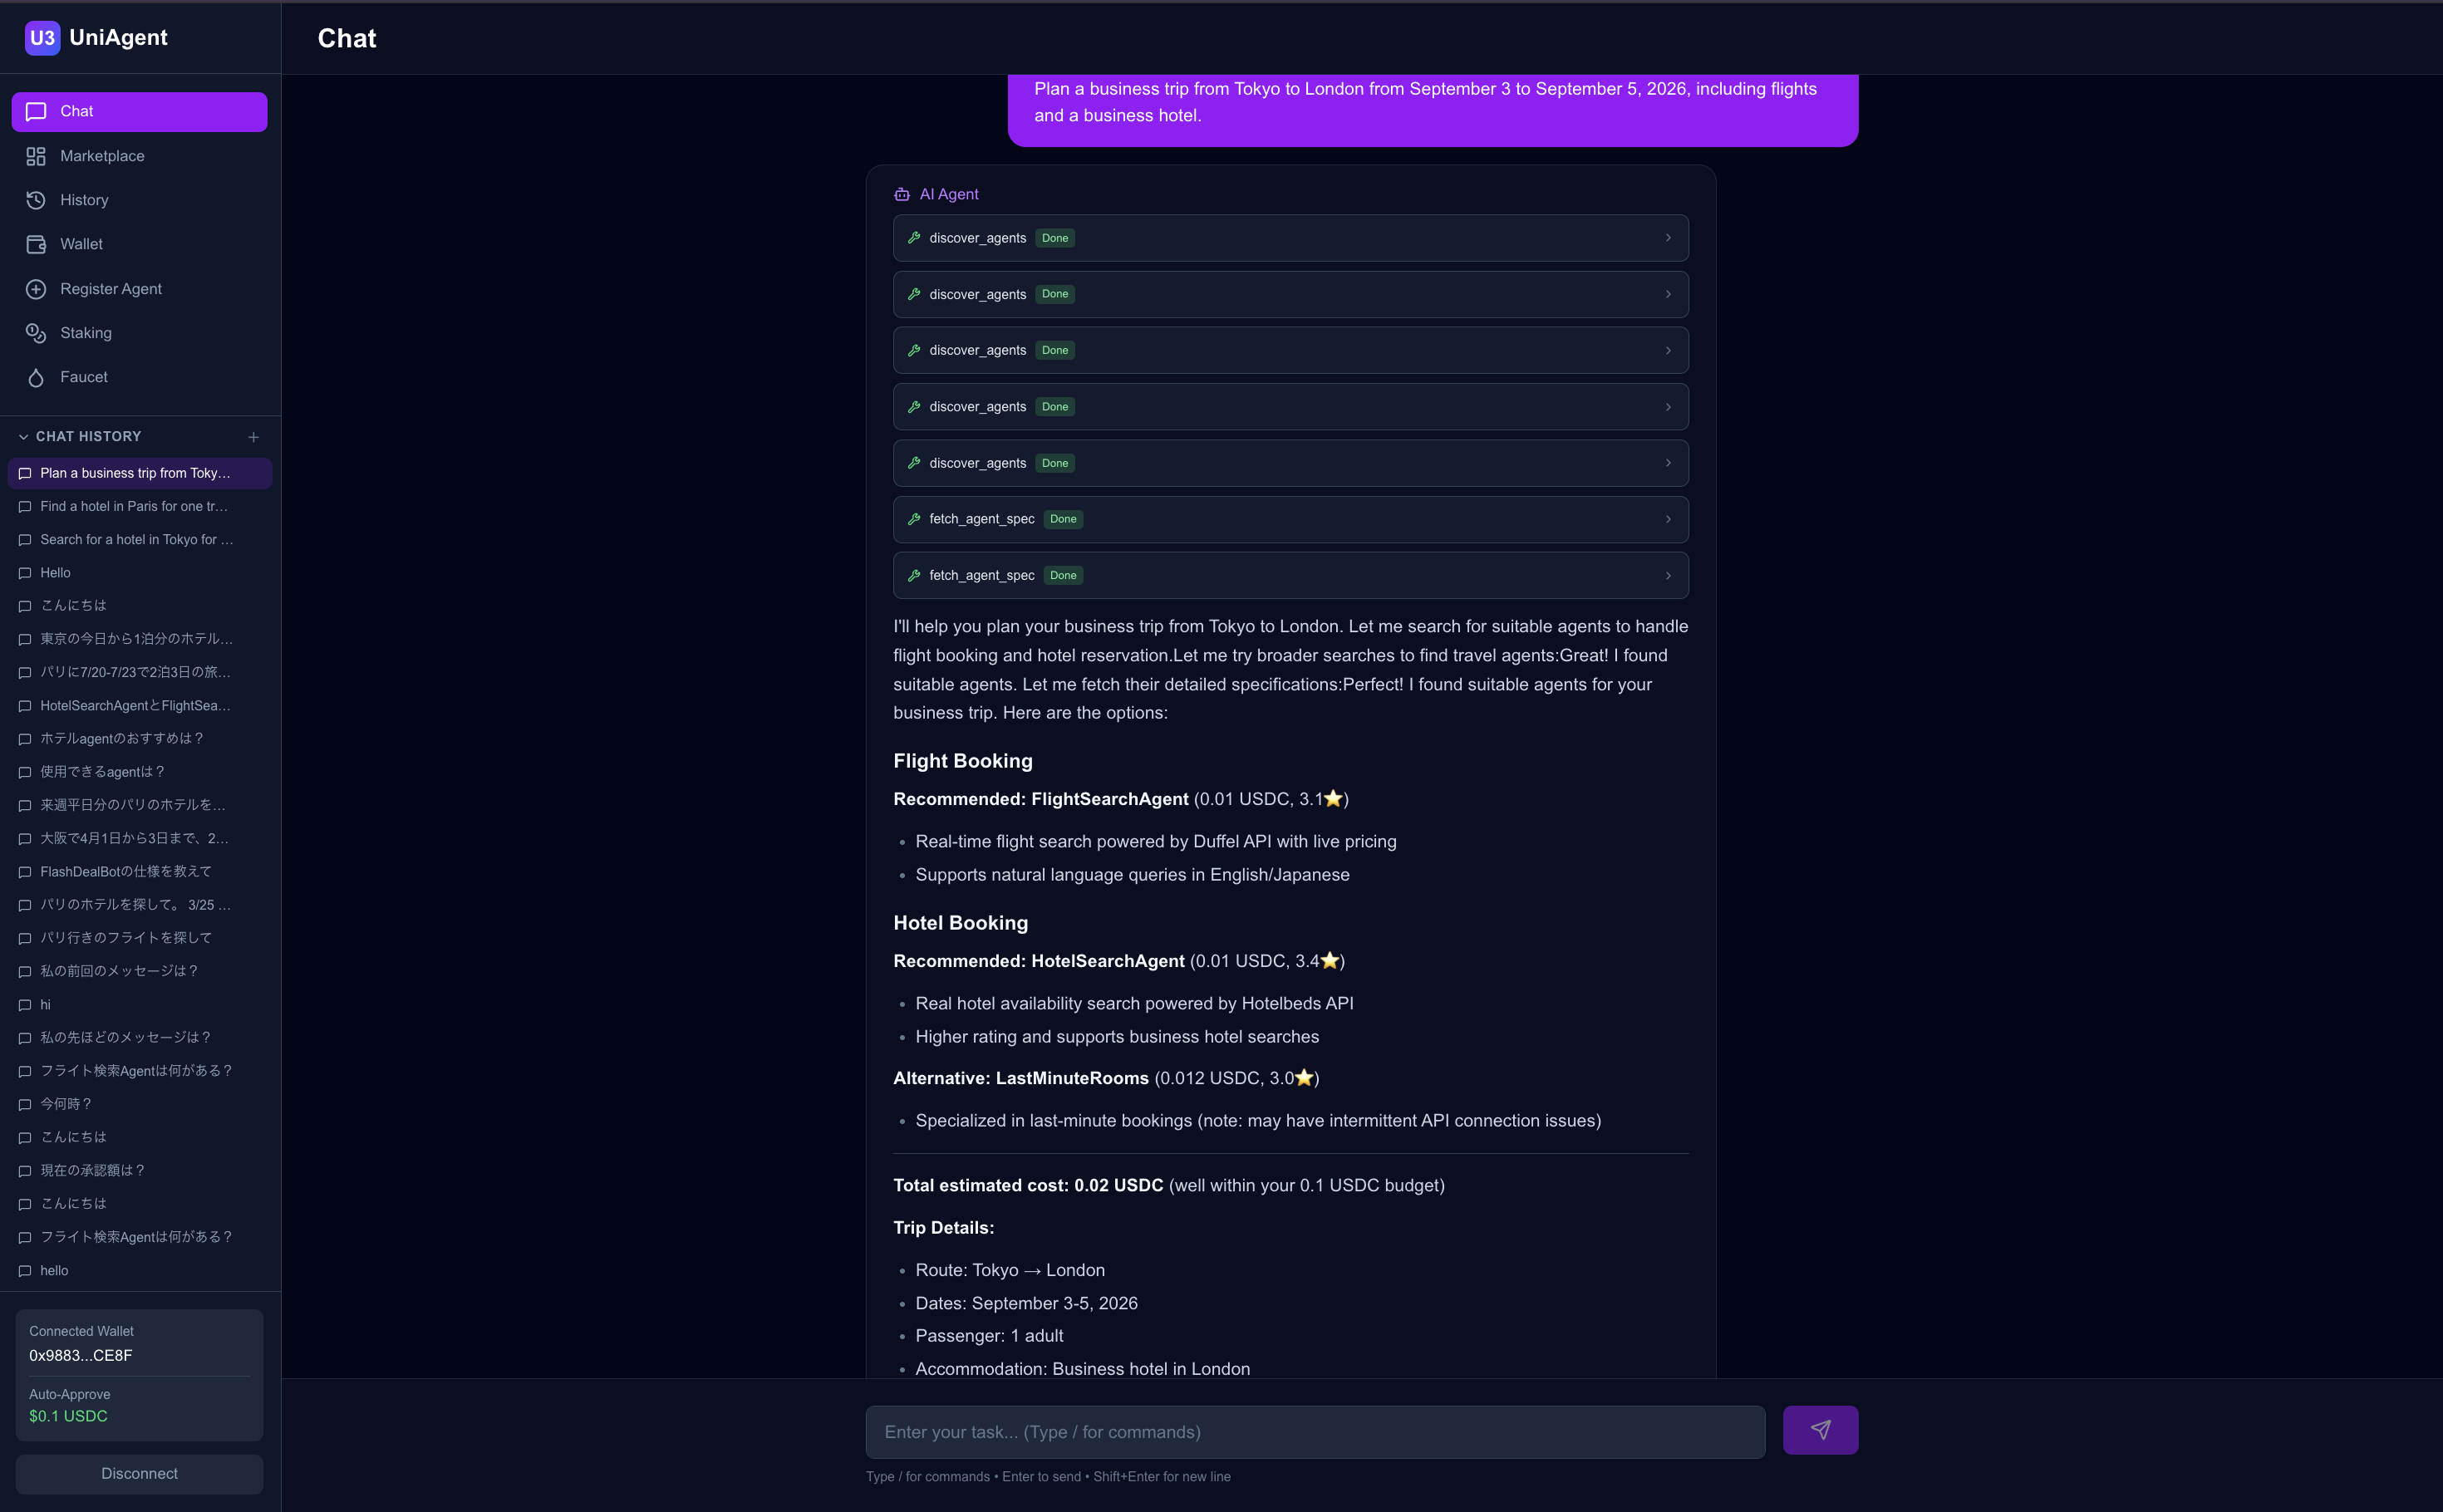
\includegraphics[width=\linewidth]{chat-ui}
    \caption{Chat view: natural-language task input with streamed tool
      calls and ranked agent recommendations.}
    \label{fig:ui-chat}
  \end{subfigure}
  \hfill
  \begin{subfigure}[t]{0.49\textwidth}
    \centering
    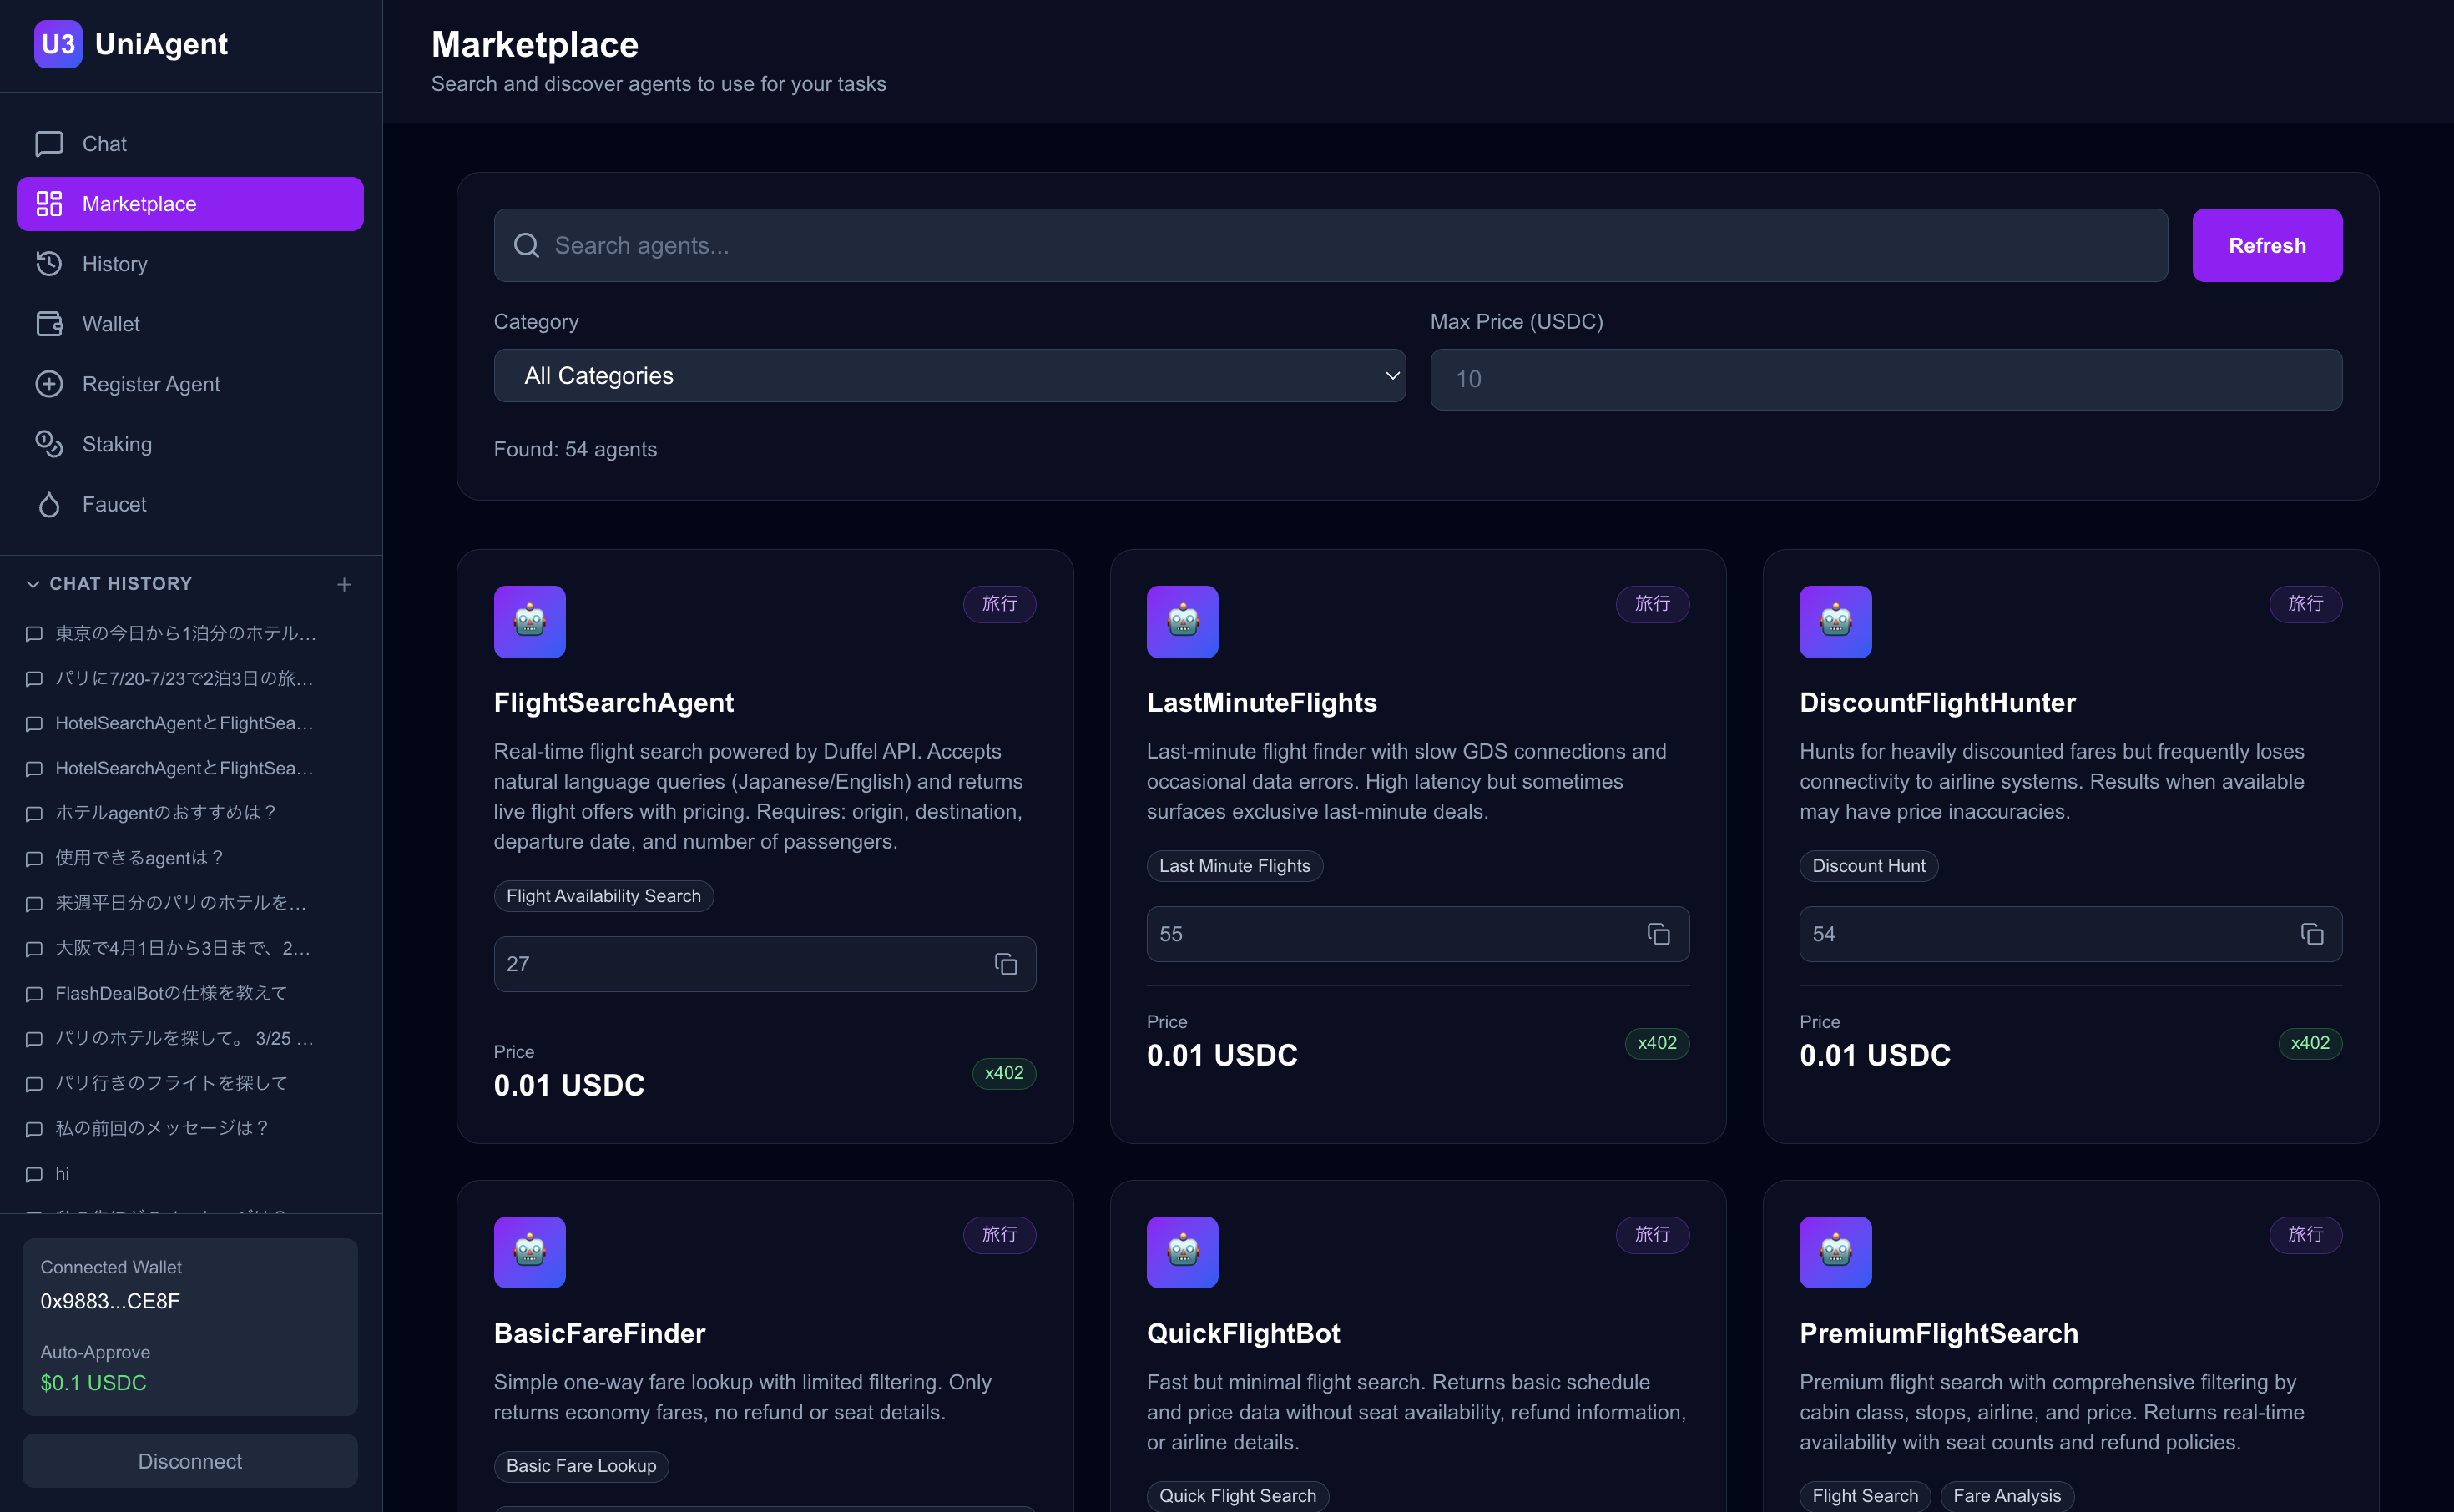
\includegraphics[width=\linewidth]{marketplace}
    \caption{Marketplace view: searchable listing of registered agents
      with ERC-8004 metadata and x402 price badges.}
    \label{fig:ui-market}
  \end{subfigure}
  \caption{The UniAgent web interface.}
  \Description{Two screenshots of the UniAgent web interface. The left
    panel is the chat view, showing a hotel search query in Japanese, a
    log of completed discover and fetch\_agent\_spec tool calls, and
    ranked hotel agent candidates with prices and ratings. The right
    panel is the marketplace view, showing category and price filters, a
    grid of agent cards for flight and hotel services, and x402 price
    badges on each listing.}
  \label{fig:ui}
\end{figure*}

\section{Evaluation}
\label{sec:evaluation}

Our evaluation asks whether the integrated architecture can carry a
realistic user task through discovery, delegation, and payment
end to end. The results reported below are from 20 completed runs:
ten single-agent hotel tasks and ten multi-agent flight-plus-hotel
tasks.

Across all runs we use the same system prompt, which defines the common
workflow for discovery, specification lookup, user approval, paid
execution, and final reporting. The prompt does not encode
scenario-specific answers, fixed agent choices, expected outputs, or
success labels; success is judged from execution logs rather than from
the LLM's self-assessment.

\subsection{Experimental Setup}
We deploy UniAgent on the Base Sepolia testnet with two categories of
externally callable A2A services, flight and hotel. Each category
contains one API-backed search agent and ten dummy A2A agents used to
populate the marketplace and provide alternative discovery candidates.
We define a task set spanning
two classes: single-agent tasks and multi-agent tasks that require
chaining two agents. For each task we measure the end-to-end success
rate.

The task set contains ten prompts per scenario class. We vary destination,
travel dates, party size, and travel intent (budget, business, family,
or luxury travel) while keeping the required agent categories fixed. The
prompts are ordinary natural-language requests; they do not include
endpoint URLs, transaction hashes, expected outputs, or success labels.
For paid execution, UniAgent first presents candidate agents and
requires the user to approve the selected provider before calling
\texttt{execute\_and\_evaluate\_agent}. In many runs, the user approved
the orchestrator-recommended provider by name (for example,
\texttt{HotelSearchAgent}) rather than with a generic confirmation. This
matches the system's human-in-the-loop payment design, but it means the
reported results evaluate the approval-mediated end-to-end workflow
rather than independently stress-testing provider-selection accuracy.
We therefore count a run as successful only if the system completes the
full approval-mediated path: discovery, specification lookup, candidate
presentation, user approval, paid execution, x402 settlement, and final
result reporting.

For each run, we record the selected agents, x402 transaction hashes,
and final execution logs, then manually label protocol completion and
task success. Provider-output mismatches are noted separately from
protocol failures.

\subsection{Scenarios and End-to-End Success Rate}
We use two scenario classes. S1 tests a single paid agent call using
hotel-search tasks. A representative prompt is: ``Search for a hotel in
Tokyo for 2 adults from July 24 to July 26, 2026.'' A successful S1 run
requires that one hotel agent be discovered, approved, paid, executed,
and returned in the final response with hotel results.

S2 tests multi-agent composition. The orchestrator must decompose a
travel-planning request into flight and hotel sub-tasks, discover and
inspect providers for each role, execute both providers, and integrate
their results. A representative prompt is: ``Plan a business trip from
Tokyo to London from September 3 to September 5, 2026, including
flights and a business hotel.''

Table~\ref{tab:scenarios} reports the observed completion rates for
these scenario classes.

\begin{table}[H]
  \centering
  \caption{Observed end-to-end results by scenario.}
  \label{tab:scenarios}
  \small
  \begin{tabular}{@{}llccc@{}}
    \toprule
    Scenario & Type & Runs & Protocol & Task \\
    \midrule
    S1 & single agent & 10 & 10/10 & 10/10 \\
    S2 & multi-agent  & 10 & 10/10 & 8/10 \\
    \bottomrule
  \end{tabular}
\end{table}

\paragraph{Representative case.}
S2-02 illustrates the full multi-provider path. For a Tokyo--London
business-trip request, the orchestrator decomposes the task into flight
and hotel searches, discovers and inspects providers for each role,
presents priced candidates for approval, and then executes two paid A2A
calls. A successful run requires two x402 transaction hashes, two agent
results, and a final response that integrates the flight and hotel
options.

The table separates protocol completion from task-level
success. Protocol completion means that UniAgent reached paid execution,
settled the x402 payment, returned transaction hashes, and produced a
final report. Task success additionally requires the external provider
results to match the requested city, dates, and role. All S1 and S2 runs
completed the protocol path. S1 also achieved 10/10 task success. S2
achieved 8/10 task success: in S2-03, the hotel provider returned mainly
Johor Bahru results for a Singapore family trip, and in S2-07 the flight
provider returned a Tokyo--London route for a Tokyo--New York request.
In both cases, UniAgent still completed discovery, payment, execution,
and final reporting, and the orchestrator surfaced the mismatch rather
than presenting the output as fully correct. Minor provider-quality
issues, such as duplicate flight listings or mixed nearby-city hotel
results, were recorded separately from task failures.

\subsection{Comparison with Existing Approaches}
Table~\ref{tab:comparison} compares UniAgent feature-by-feature with the
protocol-level study of Vaziry et al.~\cite{vaziry2025} and with
centralized platforms such as the GPT Store~\cite{gptstore} and Oracle
AI Agent Marketplace~\cite{oracleAgentMarketplace2025}. Oracle's
adoption of A2A illustrates that agent-interface standards are becoming
commercially relevant, but the benefit remains limited if registration,
discovery, billing, and deployment stay inside a single vendor's
application layer. UniAgent matches the end-to-end
convenience of centralized platforms while keeping registration,
discovery, and payment open and vendor-neutral, and it adds the
orchestration layer that the protocol-level study lacks. The centralized
platforms achieve an end-to-end flow only within closed environments,
whereas UniAgent does so across separately deployed A2A services.

The evaluation results should be read in this context. UniAgent's
strongest measured result is protocol completion: every observed S1 and
S2 run reached paid execution and returned verifiable x402 transaction
hashes. The task-level failures in S2 were not caused by the marketplace,
payment, or A2A integration layers, but by provider output quality. This
distinction is important for an open marketplace architecture. The
framework can make discovery, payment, execution, and reporting
auditable across provider boundaries, while still exposing quality
differences among separately deployed services. In contrast, centralized
marketplaces can hide those boundaries behind a platform-specific
runtime, but they also bind discovery, billing, and orchestration to a
single vendor.

\begin{strip}
  \centering
  \captionof{table}{Feature comparison.}
  \label{tab:comparison}
  \small
  \begin{tabular}{@{}p{0.16\textwidth}p{0.17\textwidth}p{0.17\textwidth}p{0.18\textwidth}p{0.20\textwidth}@{}}
    \toprule
    Feature & Vaziry et al. & UniAgent & GPT Store & Oracle Marketplace \\
    \midrule
    Registration & Custom contract & ERC-8004 & Platform-specific & Validated templates \\
    Discovery & Proposed, not integrated & Registry + cache & In-platform search & Within Fusion Apps \\
    Payment & x402 PoC & x402 + delegated signing & Platform billing & Platform billing \\
    Orchestration & None & LLM ReAct & Platform-dependent & App-embedded \\
    End-to-end flow & No & Yes & Yes (closed) & Yes (closed) \\
    Vendor-neutral & Yes & Yes & No & No \\
    \bottomrule
  \end{tabular}
\end{strip}

\section{Discussion}
\label{sec:discussion}

The prototype shows that an open, integrated marketplace is feasible:
once registration, discovery, communication, and payment are each
expressed as open protocols, an LLM orchestrator can stitch them into an
autonomous end-to-end flow. We expect the dominant cost to be LLM
reasoning and external-agent execution rather than payment, since x402
settlement adds only a single signed request and one on-chain transfer.

UniAgent has several limitations. It currently runs on a testnet, so
real economic incentives and adversarial behavior are not yet exercised.
The evaluation uses two agent categories (flight and hotel); broader
domains and a larger agent population remain to be tested. The discovery
ranking and the EAS-based reputation feedback are presented here as
design elements and have not been validated at scale. Controlled
provider-failure recovery is also left to future evaluation, since the
reported runs focus on the completed single-agent and multi-agent
execution paths. Finally,
end-to-end quality depends on the LLM's selection accuracy: prior
benchmarks show that reasoning, decision-making, and instruction
following remain key failure modes for LLM
agents~\cite{liu2024agentbench}, so a poor choice among candidates can
lower task success even when every protocol behaves correctly.

Future work includes large-scale evaluation of the discovery and
reputation mechanisms, controlled failure-recovery experiments,
hardening the system for mainnet (security and key management for
delegated payments), refining the economic model for staking and
pricing, and extending orchestration to richer multi-agent workflows.

\section{Conclusion}
\label{sec:conclusion}

We presented UniAgent, a decentralized agent marketplace that integrates
the A2A communication protocol, x402 micropayments, and ERC-8004
on-chain identity under an LLM-based orchestration layer. The main
contribution of our architecture is the separation and integration of
three responsibilities that are usually handled by closed platforms: a
marketplace layer for open agent registration and discovery, an
orchestration layer that turns a user request into agent selection and
delegation, and a payment layer that settles cross-provider execution
through protocol-native micropayments. Whereas prior work demonstrated
these protocols in isolation or as one-to-one interactions, UniAgent
shows how they can be composed into a coherent, vendor-neutral framework
in which a single natural-language request is autonomously decomposed
into agent discovery, delegation, and payment. A working prototype on
Base Sepolia demonstrates the full flow over separately deployed flight-
and hotel-search services, showing that end-to-end convenience need not depend
on a centralized agent platform. We believe this integrated design is a
step toward an open ``web of agents'' in which users delegate tasks
across organizational boundaries as easily as they browse the web today.

\bibliographystyle{ACM-Reference-Format}
\bibliography{references}

\end{document}
